\chapter{Тест Колмогорова-Смирнова}
\label{ch:сhap5}

\textbf{Теория:}

Критерий Колмогорова-Смирнова является непараметрическим статистическим критерием, используемым для проверки гипотез о законе 
распределения генеральной совокупности или о равенстве законов распределения двух генеральных совокупностей. То есть данный 
тест позволяет проверить, принадлежит ли заданная выборка некоторому теоретическому распределению. \\

Для проверки работы критерия сгенерируем в MATLAB выборку из экспоненциального распределения и проверим, можно ли её считать 
выборкой из стандартного нормального распределения.

Реализация:


\begin{figure}[H]
    \centering
    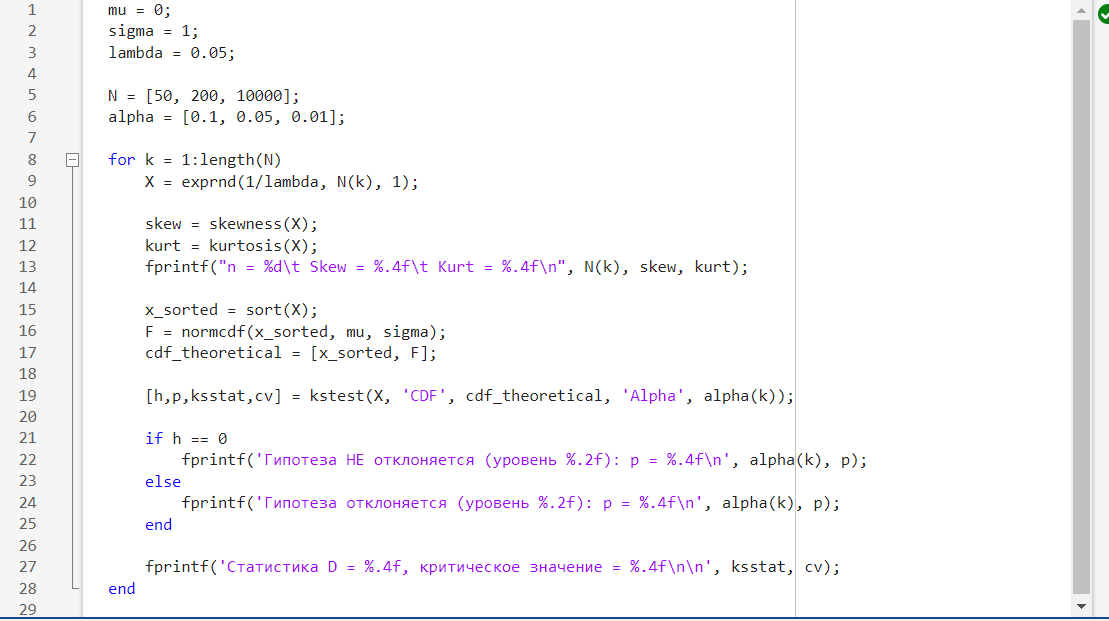
\includegraphics[width=1.0\textwidth]{colm_test.png}
    \caption{Пример использования теста Колмогорова-Смирнова}
\end{figure}


Результат:

\begin{figure}[H]
    \centering
    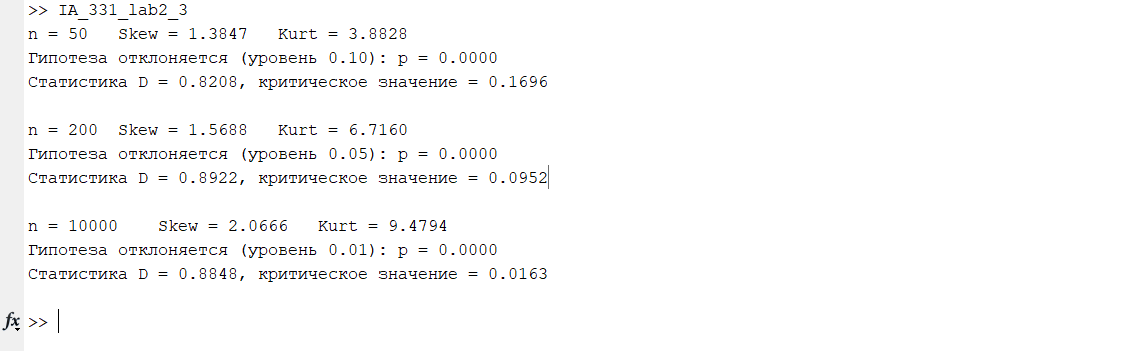
\includegraphics[width=1.0\textwidth]{colm_res.png}
    \caption{Результат использования теста Колмогорова-Смирнова}
\end{figure}

\textbf{Вывод:} \\

Тест показывает, что выборка из экспоненциального распределения не является выборкой из нормального стандартного распределения,
что логично.

\endinput